\subsection{General Architecture}
	To develop the system, we will be continuing with the Django Web Framework. We are utilising this framework to continue development as well as meet the requirement of it being specifically developed in Django. Django implements the Model View Controller (MVC) software architecture for developing systems. While it does not utilise the same names, it still maintains this structure. We will be implementing this exact model that Django utilises by following its recommended method to enforce this model. Django refers itself as a Model View Template framework to refer to the naming convention it utilises.\\
		
		\noindent The MVC model is an architecture that aims at delivering objects or interfaces by separating the data into three components, this being the model, view and controller. Each one of these components has a separate task, which is either independent from other applications or weekly coupled to the other components.\\
		
		%%%%%%%%%%%%%%%%%%%%%%%%%
		%  Django MVC Model	
		%%%%%%%%%%%%%%%%%%%%%%%%%
		\subsubsection{Abstract View of  a CAMEL Application}	
		\begin{figure}[h]
			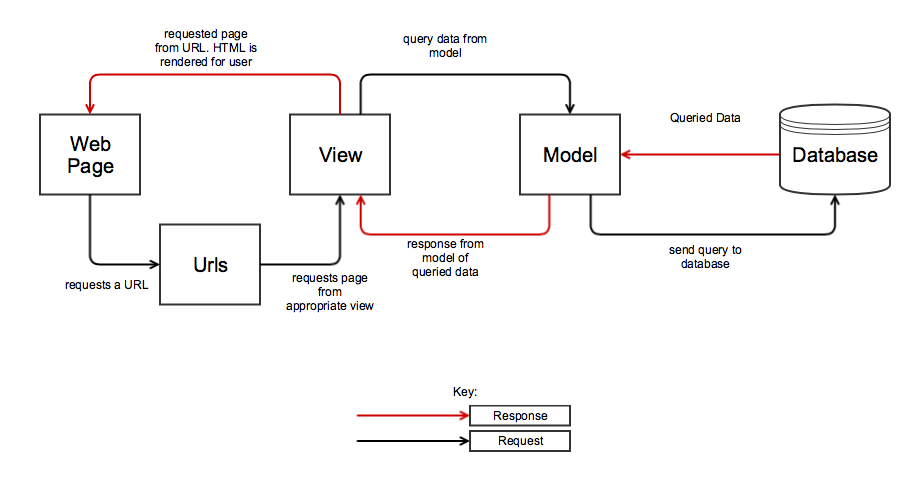
\includegraphics[scale=0.40]{softwarearchitecture/img/caml_mvc_abstract_diagram}
			\caption{Django Model View Controller Design}
			\centering
		\end{figure}
		
		The flow of the diagram is that when a web page is requested by the user via the URL, the URL file will redirect this to a view file. This file is the controller that will look at the request, and obtain any models to complete the request. The models will then pull data about itself from the database, which is then passed to the view function. The view will then finally return the page that the user requested along with any model data it need. The view will render the HTML and Django template language to create the final web page that the user interacts with. The rendering of the page allows the template to be re-used to provide different content.\\ 		
		
		Our system will comprise of a number of these applications that will complete the final system. As a group, we have decided to ensure that we can make each application be de-coupled as much as possible. This was a design choice to allow for future flexibility when development continues after us as the applications have re-usability in mind when it was developed. Additionally, by having the applications created that are highly cohesive, it ensures that the requirement of splitting the applications down is met.\\
		
		The final CAMEL application will be partitioning the original 'core' file into separate applications. These applications will be: core, module, homework, user and review.\\
		
		The main motivation that 'core' was separated is to allow the applications to be de-coupled from each other. By having the applications de-coupled, it allows for high re-usability as the application can be re-used again. This allowed the applications to support the notion of being open source, as allowing it to be removed from the system with ease and used by anyone. Further reasons that we chose to de-couple the code was to allow for better black box re-use. As the code was placed in specialised files, it allowed only the relevant methods to be obtained and used. This allows for a better understanding by developers, as methods that are imported are the only ones that will be utilised. It also makes the code more cohesive, as it will only do a specific function or type. For example, only code related to the module is kept in this application, so a developer knows where the resource related to modules is located.\\   